\documentclass{article}
\usepackage{graphicx,booktabs,hyperref}
\ifdefined\anonymouspaper
  \usepackage{icml2027}
\else
  \usepackage[preprint]{icml2027}
\fi
\usepackage{iftex}
\ifPDFTeX
  \usepackage{times}
\else
  \usepackage{fontspec}
  \setmainfont{NimbusRoman-Regular.otf}[
    Path = fonts/,
    BoldFont = NimbusRoman-Bold.otf,
    ItalicFont = NimbusRoman-Italic.otf,
    BoldItalicFont = NimbusRoman-BoldItalic.otf
  ]
\fi
\usepackage{amsmath,amssymb,array,xcolor,url,tikz}
\usetikzlibrary{arrows.meta,positioning}
% ICML hides the margin ruler in preprint mode. Keep the supplied ruler
% visible in the named project copy as well; review mode already supplies it.
\ifdefined\anonymouspaper\else
\AddToShipoutPicture{%
  \icmlruleroffset=\textheight
  \advance\icmlruleroffset by 5.2pt
  \color[rgb]{.7,.7,.7}%
  \AtTextUpperLeft{\put(\LenToUnit{-35pt},\LenToUnit{-\icmlruleroffset}){\icmlruler{\icmlrulercount}}}%
}
\fi
\icmltitlerunning{Which Exposure Matters?}
\begin{document}
\twocolumn[
\icmltitle{\texorpdfstring{\LARGE Which Exposure Matters?\\Design Diagnostics and Diffusion Model Feasibility}{Which Exposure Matters? Design Diagnostics and Diffusion Model Feasibility}}
\begin{icmlauthorlist}
\icmlauthor{Kanishak Mittal}{iiit}
\icmlauthor{Aryan Tripathi}{iiit}
\icmlauthor{Nikhil Tomar}{iiit}
\icmlauthor{Vansh Rathore}{iiit}
\end{icmlauthorlist}
\icmlaffiliation{iiit}{Indian Institute of Information Technology Raichur, India}
\icmlcorrespondingauthor{Kanishak Mittal}{cs24b1017@iiitr.ac.in}
\icmlcorrespondingauthor{Aryan Tripathi}{ad24b1010@iiitr.ac.in}
\icmlcorrespondingauthor{Nikhil Tomar}{cs24b1041@iiitr.ac.in}
\icmlcorrespondingauthor{Vansh Rathore}{cs24b1061@iiitr.ac.in}
\icmlkeywords{Diffusion Models, Compositionality, Exposure, Evaluation}
\vskip 0.3in
]
\printAffiliationsAndNotice{}
\begin{abstract}
Diffusion models can draw familiar objects yet fail to combine their attributes and spatial relationships. We ask whether composition success is associated with exposure to the complete combination beyond exposure to its individual predicates. We propose a controlled synthetic-scene framework: estimate the exposure of primitive predicates and their conjunctions, optimize training mixtures while monitoring confounding, train conditional diffusion models, and evaluate with human-audited predicate checks. In an initial feasibility block, four small models trained for 500,000 updates each on 200 images per condition generated 64 preselected images. Human labels mark 59 requested-color circles present, three absent and two unresolved. Finite-image bounds for the complexity drop are 0.0625--0.125; the corresponding imbalance drop is $-0.03125$--0.03125. These bounds are not confidence intervals. A second training-seed block on the same dataset gives a zero descriptive complexity drop. The checker frequently abstains, and identical returned review files cannot independently establish reviewer identities. The work is an instrument-development study, not a completed causal finding or an established replication.
\end{abstract}
\section{Introduction}
A generative image model may know what ``red'', ``circle'', and ``left of'' mean individually but still place the wrong color on an object or reverse a relation. Such errors reveal a gap between learning concepts and composing them. Diffusion models learn by corrupting training images with noise and learning to reverse that corruption. Their success depends partly on what training examples show together, yet the frequency of a complete configuration is entangled with the frequencies of its ingredients.

\textbf{Research question.} When a model sees the individual ingredients often, does additional exposure to their particular combination predict success on that combination? Our hypothesis is that joint exposure carries information beyond individual exposure and rule complexity, when these quantities can be varied and measured independently. The study is designed to test this hypothesis; the present results do not establish it.

Our contribution is a \emph{proposed} controlled intervention and measurement pipeline combining predicate-level semantics, exposure matrices, constrained mixture design, identifiability diagnostics and human-audited generation checks. The individual ideas and synthetic data are not claimed as new in isolation. The current empirical contributions are a 5.7-million-scene exposure measurement and a small matched four-condition model-feasibility experiment.
\section{Literature Survey}
Denoising diffusion probabilistic models (DDPMs) learn a sequence of noise-removal steps \cite{ho2020}. Latent diffusion scales generation by denoising in a learned compressed representation \cite{rombach2022}. Liu et al. compose diffusion models at inference time \cite{liu2022}, while Liang et al. examine factorized representations in controlled diffusion experiments \cite{liang2024}. Okawa et al. study how compositional abilities emerge with data frequency on a synthetic task \cite{okawa2023}; Jeong et al. directly study object complexity and concept imbalance \cite{jeong2026}. T2I-CompBench evaluates attribute binding, relations and complex combinations \cite{huang2023}. These works already establish the importance of composition, frequency and controlled synthetic experiments. Our gap is the planned \emph{joint} examination of marginal versus conjunction exposure under explicit mixture constraints and auditable rule semantics, not the first observation that frequency matters.

\begin{table*}[t]\centering\small
\caption{Selected related work. Published task metrics are not directly comparable to our synthetic pilot; no numerical cross-study ranking is implied.}
\begin{tabular}{p{2.0cm}p{3.2cm}p{2.5cm}p{2.7cm}p{3.8cm}}\toprule
Work & Method & Reported performance / scope & Data & Critical remark \\\midrule
Rombach et al. (2022) \cite{rombach2022} & Latent-space diffusion with conditioning & High-resolution synthesis & Multiple image benchmarks & Improves synthesis, not a controlled causal exposure study \\
Okawa et al. (2023) \cite{okawa2023} & Synthetic compositional diffusion task & Studies frequency-dependent compositional emergence & Controlled synthetic data & Closely related; frequency and multiplicative structure are not novel to us \\
Huang et al. (2023) \cite{huang2023} & Compositional benchmark & 6,000 prompts across composition categories & T2I-CompBench prompts & Evaluates models rather than controlling their training exposure \\
Jeong et al. (2026) \cite{jeong2026} & MOSAIC multi-object study & Examines imbalance and complexity & Controlled multi-object setup & Our four-cell toy study is an adaptation, not their full replication \\\bottomrule
\end{tabular}\end{table*}

\section{Methodology}
\subsection{Diffusion in brief}
For a clean training image $x_0$, a forward process forms $x_t=\sqrt{\bar\alpha_t}x_0+\sqrt{1-\bar\alpha_t}\epsilon$, with $\epsilon\sim\mathcal N(0,I)$. A conditional neural network learns a denoising target at many timesteps. Velocity prediction follows \cite{salimans2022}, and condition dropout follows classifier-free guidance \cite{ho2022}. At generation time it starts with noise and iteratively reverses the process, conditioned on the requested color. The visual noising sequence in Figure~\ref{fig:noising} gives intuition but is not a sampled DDPM schedule. Our PilotUNet uses a velocity-prediction objective; this is a small pixel-space conditional network, not a pretrained text-to-image model. Figure~\ref{fig:flow} separates training, generation and measurement.
\paragraph{The denoising optimization.} Let $a_t=\bar\alpha_t$ and let $\tilde c$ be either the requested color or the null condition under training-time condition dropout. The velocity target and the objective used in the pilot are
\begin{align}
 v_t &= \sqrt{a_t}\,\epsilon-\sqrt{1-a_t}\,x_0,\\
 \mathcal L(\theta)&=\mathbb E_{x_0,c,t,\epsilon}
 \left[\lVert v_\theta(x_t,t,\tilde c)-v_t\rVert_2^2\right].
\end{align}
The expectation is approximated by minibatches of training images, uniformly selected timesteps and independent Gaussian noise; the pilot uses a linear noise schedule from $10^{-4}$ to $0.02$ over 1,000 steps; AdamW updates the network parameters. At sampling time the predicted velocity is converted to a predicted noise vector by
\begin{equation}
 \hat\epsilon_t=\sqrt{a_t}\,v_\theta(x_t,t,c)
 +\sqrt{1-a_t}\,x_t.
\end{equation}
With the convention $\hat v=v_{\varnothing}+g(v_c-v_{\varnothing})$, guidance $g=1$ gives $\hat v=v_c$; it does not amplify the conditional direction. The pilot used condition dropout 0.1, AdamW learning rate $10^{-4}$ and EMA decay 0.999. This conversion is an algebraic identity when the velocity prediction is exact; a low training loss alone does not establish conditional generation success.

\begin{figure*}[t]\centering
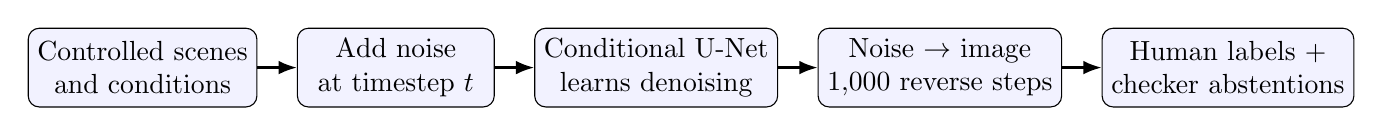
\begin{tikzpicture}[node distance=5mm, box/.style={draw,rounded corners,align=center,minimum height=10mm,minimum width=25mm,fill=blue!5},>=Latex]
\node[box](data){Controlled scenes\\and conditions}; \node[box,right=of data](noise){Add noise\\at timestep $t$}; \node[box,right=of noise](net){Conditional U-Net\\learns denoising}; \node[box,right=of net](sample){Noise $\rightarrow$ image\\1,000 reverse steps}; \node[box,right=of sample](audit){Human labels +\\checker abstentions};
\draw[->,thick](data)--(noise);\draw[->,thick](noise)--(net);\draw[->,thick](net)--(sample);\draw[->,thick](sample)--(audit);
\end{tikzpicture}
\caption{The completed model-feasibility workflow. The proposed exposure-mixture intervention precedes model training and remains under design validation.}\label{fig:flow}\end{figure*}
\begin{figure}[t]\centering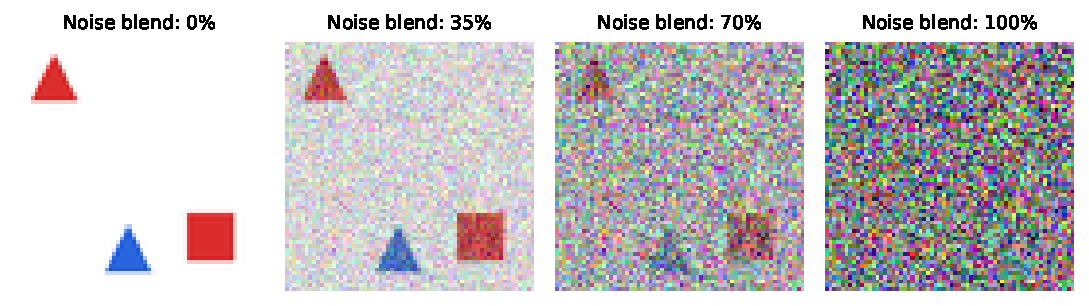
\includegraphics[width=\columnwidth]{figures/illustrative-noising.pdf}\caption{Illustrative Gaussian-blend sequence, shown from image to noise. It is not a model output or the actual DDPM schedule.}\label{fig:noising}\end{figure}
\subsection{Exposure and controlled intervention}
Represent a rule $r$ as a conjunction of predicates $p\in r$, such as a color and a shape bound to an object, or a relation between distinct objects. For each training condition $j$, estimate $A_{pj}=P_j(p)$ and $A_{rj}=P_j(r)$. A mixture with weights $w_j\ge0$, $\sum_j w_j=1$, has marginal exposure $m_p=\sum_j w_jA_{pj}$ and joint exposure $n_r=\sum_jw_jA_{rj}$. A descriptive joint-exposure lift is $\ell_r=\log n_r-\sum_{p\in r}\log m_p$ when all terms are positive. Mixtures can be optimized to vary $\ell_r$ while approximately preserving specified marginal exposures. Sampling uncertainty matters: estimated constraints do not imply exact population equality. The illustrative example in Figure~\ref{fig:joint} shows why matching marginal frequencies does not fix joint exposure. A scene-level existential singleton and a same-object conjunction are different events: the product of singleton probabilities is not in general the probability of the bound rule.
\begin{figure}[t]\centering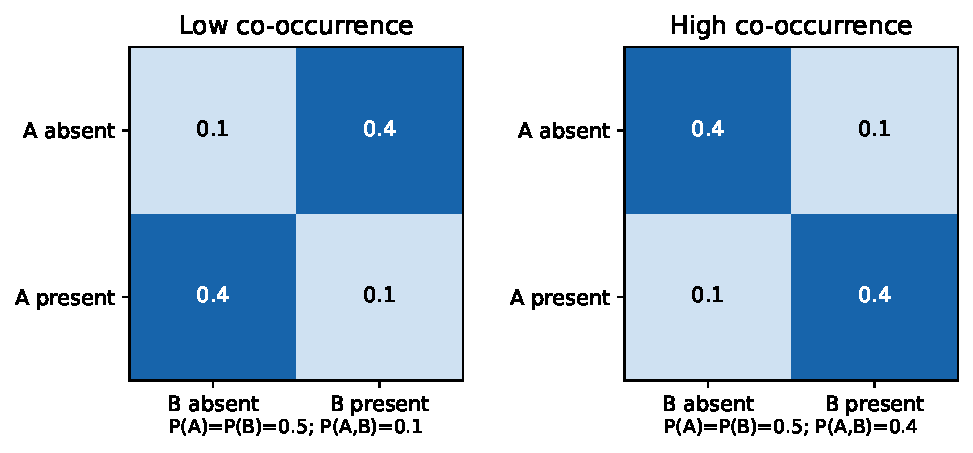
\includegraphics[width=\columnwidth]{figures/marginals-joint-example.pdf}\caption{Constructed example, not measured data: two distributions have identical marginals but different joint exposure.}\label{fig:joint}\end{figure}

A separate planned outcome, rule satisfaction rate (RSR), is the proportion of generated outputs satisfying $r$. One proposed interaction index is $\Gamma_r=\operatorname{logit}(\mathrm{RSR}_r)-\operatorname{logit}(\prod_{p\in r}c_p)$, where $c_p$ is the corresponding primitive success rate. Under $\mathrm{RSR}_r=\prod_pc_p$, $\Gamma_r=0$. This baseline is a diagnostic, not proof of independence or causality. Rule-level intercepts can make effects of a within-rule constant marginal unidentifiable; pooled correlations alone do not repair that problem.
\subsection{Constrained mixture optimization}
For $J$ candidate training conditions, let $\widehat A_{ej}$ be the estimated probability of event $e$ under condition $j$ and let $w_j$ be its mixture weight. The estimates are empirical averages of event indicators over accepted scenes:
\begin{equation}
 \widehat A_{ej}=\frac{1}{N_j}\sum_{i=1}^{N_j}
 \mathbf 1\{e\text{ holds in scene }i\text{ of }j\}.
\end{equation}
For specified lower and upper exposure bounds $L_e,U_e$, the implemented feasible set is
\begin{align}
 \widehat{\mathcal W}=\{w\in\mathbb R^J:\;&\mathbf 1^\top w=1,\quad w_j\geq w_{\min},\notag\\
 &L_e\leq\widehat A_{e:}w\leq U_e\quad\forall e\}.
 \label{eq:feasible}
\end{align}
Here $e$ may denote a complete rule, an individual predicate or an indicated predicate pair. Finding any $w\in\widehat{\mathcal W}$ is a linear feasibility problem. When the uniform reference $u_j=1/J$ is feasible, the optional minimum-KL design solves
\begin{equation}
 \min_{w\in\widehat{\mathcal W}}D_{\mathrm{KL}}(w\Vert u)
 =\min_{w\in\widehat{\mathcal W}}\sum_{j=1}^{J}w_j\log(Jw_j),
\end{equation}
with $0\log 0=0$. The objective is convex and the feasible set is defined by linear constraints. By nonnegativity of KL divergence, $u$ is its unique minimizer with value zero when feasible, so this objective alone does not generate an exposure contrast. If the constraints exclude $u$, the feasible minimum is positive. The later contrast-seeking max--min mixture design is a separate exploratory problem; it is not a demonstrated solution of this convex baseline or a passed design gate.

To obtain rule-specific extremes, the multi-matrix exploratory procedure fixes each singleton marginal to its reference value on each fitting matrix $\widehat A^{(k)}$ relative to a chosen reference $w^{\mathrm{ref}}$, and solves two linear programs:
\begin{align}
 w_r^{-},w_r^{+}&\in\arg\min_{w},\arg\max_{w}
 \;\widehat A^{(1)}_{r:}w,\quad\text{subject to} \notag\\
 \mathbf1^\top w&=1,\; w_j\geq w_{\min},\;\;\widehat A^{(k)}_{p:}w=\widehat A^{(k)}_{p:}w^{\mathrm{ref}}
 \;\;\forall p,k.\label{eq:lp}
\end{align}
The constraints preserve empirical singleton rows, not the unknown population probabilities, and the endpoints can concentrate heavily on a few conditions. Optimizing individual rule endpoints does not by itself identify a common causal coefficient or ensure that all desired covariates are decorrelated. The reported candidate and its diagnostics are exploratory.

\paragraph{Exploratory allocation diagnostics.} In a separate local search over rule-allocation weights $q$, one implemented penalty targets both collinearity and marginal--lift correlation on the fitting matrices:
\begin{align}
 F(q)=\sum_k\bigg[&\sum_h\big[\mathrm{VIF}_{kh}(q)-1.85\big]_+^2\notag\\
 &+25\big[|\rho_k(q)|-0.24\big]_+^2\bigg],
\end{align}
where $[z]_+=\max(z,0)$, $h$ indexes the specified covariates, and $\rho_k$ is the weighted correlation between log mean marginal and log lift. For a nonsingular weighted covariance matrix $\Sigma_k$, $\mathrm{VIF}_{kh}=(\Sigma_k)_{hh}(\Sigma_k^{-1})_{hh}$. The thresholds 1.85 and 0.24 are optimization margins, not acceptance thresholds; local convergence does not establish a global optimum or generalization. Changing $q$ also changes the population represented by the analysis.

For a proposed outcome model, a coefficient measuring the association of joint lift with success would require an estimable specification and overlap across designs. If the log-marginal exposure is held exactly constant within each rule, its column is a linear combination of rule indicators; a regression containing unrestricted rule intercepts cannot separately identify that effect. This rank deficiency is a design property, not a numerical optimization failure.

\subsection{Networked execution and integrity}
An experimental CPU producer streams rendered PNG scenes and JSON annotations over a framed TCP connection; an opt-in adapter supplies conditioned scenes to the pilot trainer. The client checks provenance, image hashes and rule satisfaction of the returned annotations. A separate checkpoint-transfer prototype compresses stable files, resumes from the received byte offset after interruption, and verifies compressed and decompressed SHA-256 before publication. An image-level inference prototype distributes fixed color/seed jobs to loopback TCP workers, verifies the checkpoint and returned image hashes, retries on another worker after failure, and records per-job timing. A two-image test used both GPU laptops; multi-GPU speedup and general cross-device reproducibility have not been established. The protocols assume trusted peers or an authenticated SSH tunnel: checksums detect accidental corruption but do not authenticate a sender. Independent training jobs can be assigned to separate devices without claiming synchronous distributed gradient optimization.

\subsection{Estimation and diagnostics}
A fresh renderer measurement (seed 82511) used 100,000 accepted scenes per condition across 57 rule conditions, totaling 5.7 million accepted scenes and approximately 57.8 million candidate attempts. It estimates the renderer's exposure probabilities, not real-world generalization. We assess mixture constraints, correlation and variance inflation factors (VIFs), including sensitivity to the reference group. A concentrated candidate achieved five VIFs below two and correlation 0.237, but its reference-adjusted maximum VIF was 4.887, the largest estimated marginal deviations were 0.0101 and 0.00749 for the two references, and its rule allocation changed the target population. The five covariates were log mean marginal exposure, log lift, attribute count, relation count, and log breadth; the adjusted analysis also included a reference-group indicator. Equal-rule alternatives tested also failed several VIF thresholds. These exploratory optimizations are not an impossibility proof or a passed design gate.
\section{Results and Discussion}
\subsection{Dataset and experimental setup}
The model feasibility experiment used internally generated 64$\times$64 synthetic shapes, generated for this study. Four conditions cross scene complexity (two versus three objects) with color balance (50:50 versus 90:10), with 200 fixed scenes per condition. Each condition used one matched PilotUNet model (width 16, batch size 4, 1,000 diffusion timesteps, AdamW, EMA), trained for 500,000 updates. A fixed generation protocol used EMA weights, 1,000 reverse steps, guidance 1, two requested colors, and eight paired noise seeds: 16 images per cell, 64 total. In these pilot data, target circles are always red or blue and distractors are green or yellow squares or triangles; target role is therefore confounded with attributes and both target combinations occur in training. The four datasets use sequential draws from one RNG, not matched scene geometries. Consequently the pilot does not measure novel attribute recombination or isolate complexity from all scene differences. This is not a conventional train/validation/test split: evaluation images are new model samples, not a held-out dataset. A second training-seed block was completed on the same dataset; it does not provide dataset-level replication.
\subsection{Ablation and quantitative analysis}
The four cells form a \emph{data-factor} comparison with matched model initialization and training random streams, not matched scene geometries or an architecture ablation. Attention-block or U-Net-component ablations have not been performed; no component benefit is claimed. The target is whether the requested-color circle appears. Object count is secondary and was not requested as an additional prompt.
\begin{figure}[t]\centering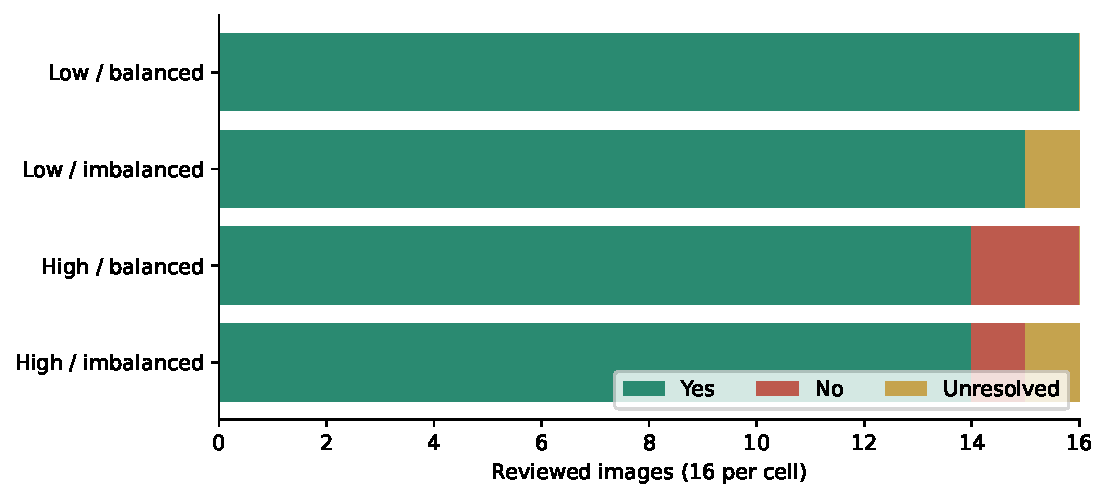
\includegraphics[width=\columnwidth]{figures/review-counts.pdf}\caption{Target-circle labels in the 64-image fixed evaluation. Four returned files were byte-identical; independent review cannot be inferred from those files.}\label{fig:counts}\end{figure}
\begin{figure}[t]\centering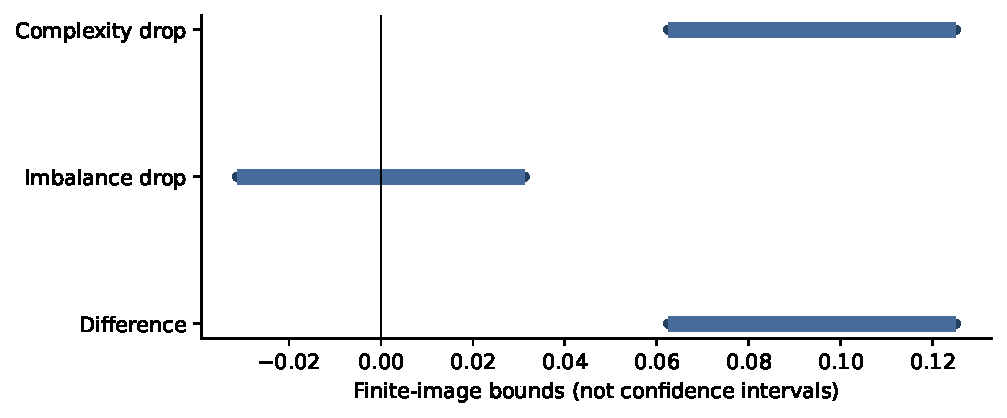
\includegraphics[width=\columnwidth]{figures/bounds.pdf}\caption{Worst-case finite-image bounds when unresolved labels are assigned either value. These are not confidence intervals.}\label{fig:bounds}\end{figure}
\begin{table}[t]\centering\small
\caption{Exact target-circle labels in the fixed 64-image evaluation. U denotes unresolved. The low/imbalanced cell has one unresolved label.}\label{tab:labels}
\begin{tabular}{lrrr}\toprule
Cell & Yes & No & U\\\midrule
Low / balanced & 16 & 0 & 0\\
Low / imbalanced & 15 & 0 & 1\\
High / balanced & 14 & 2 & 0\\
High / imbalanced & 14 & 1 & 1\\\midrule
Total & 59 & 3 & 2\\\bottomrule
\end{tabular}\end{table}
Figure~\ref{fig:colors} breaks down the same finite-image counts by requested color. Figure~\ref{fig:counts} shows 59 yes, three no and two unresolved; ``maybe'' and ``not sure'' remain unresolved. Let $s_{LB},s_{LI},s_{HB},s_{HI}$ be the four equally weighted cell success rates. Define $D_C=(s_{LB}+s_{LI}-s_{HB}-s_{HI})/2$ and $D_I=(s_{LB}+s_{HB}-s_{LI}-s_{HI})/2$; therefore $D_C-D_I=s_{LI}-s_{HB}$, not a third independent contrast. The complexity drop is bounded by 0.0625--0.125, imbalance drop by $-0.03125$--0.03125, and their difference by 0.0625--0.125 (Figure~\ref{fig:bounds}). This direction agrees with a larger complexity drop in this small block, but does not establish the population effect, a reproducible seed-level effect, or the main joint-exposure hypothesis. Noise seeds are not independent model-training replicates.

The second block has 58 yes and six no labels across 64 images, with descriptive $D_C=0$ and $D_I=-0.0625$. It shares the training dataset with the first block; two training-seed blocks and finite-image counts are insufficient to establish a population contrast. The team confirmed that its four reviews were independent, while the returned byte-identical files do not independently establish reviewer identities.
\begin{figure}[t]\centering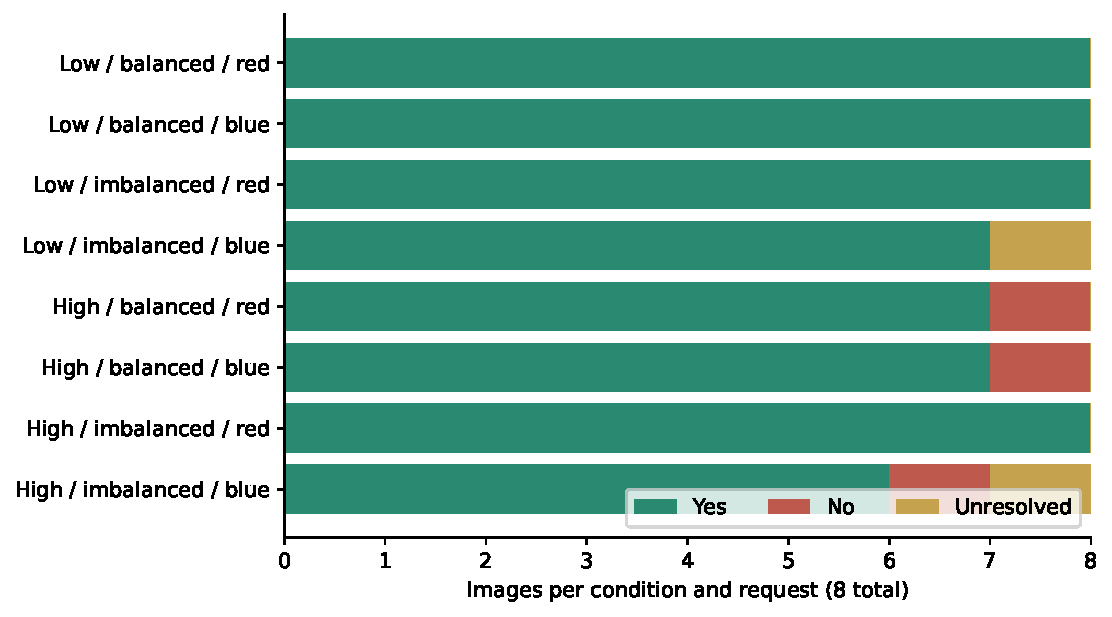
\includegraphics[width=\columnwidth]{figures/review-by-color.pdf}\caption{Requested-color circle labels by cell and color, eight images per bar. These are descriptive counts, not model-seed replication.}\label{fig:colors}\end{figure}
\subsection{Qualitative analysis and checker coverage}
\begin{figure*}[t]\centering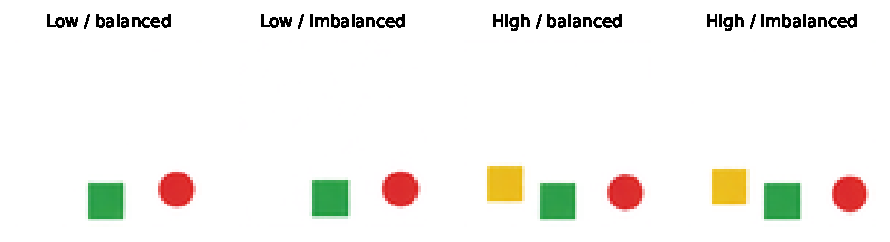
\includegraphics[width=.88\textwidth]{figures/matched-samples.pdf}\caption{Illustrative generated samples: the same red request and generation seed across the four cells. The examples use the prespecified seed 82000 and are not estimates of average quality or paired ground truth.}\label{fig:samples}\end{figure*}
Figure~\ref{fig:samples} illustrates generated outputs, not ground-truth target masks. Visual recognizability and object separation vary; they require a defined audit rather than subjective quality claims. The standard checker answered 9/64 and the experimental checker 46/64; all answered cases agreed with the labels, while 55 and 18 respectively were abstentions (Figure~\ref{fig:checker}). The experimental checker abstained on all three human-negative and both unresolved cases. Consequently these data cannot estimate its false-accept rate, and agreement among answered cases is selected-sample agreement.
\begin{figure}[t]\centering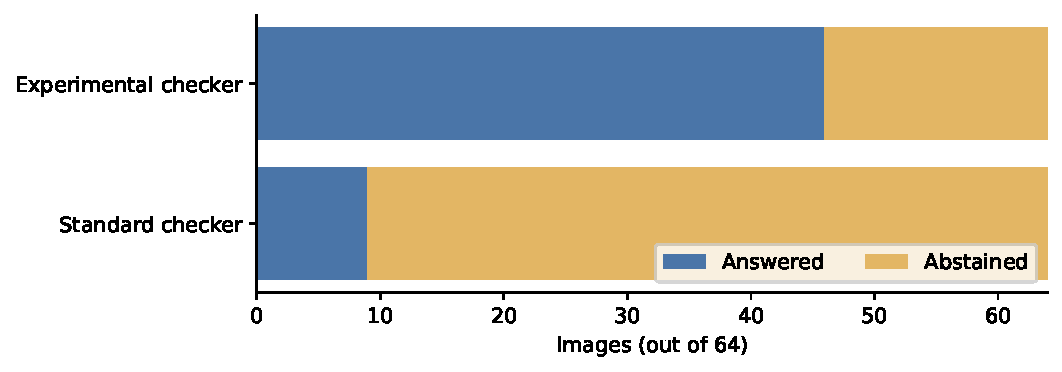
\includegraphics[width=\columnwidth]{figures/checker-coverage.pdf}\caption{Checker coverage on 64 generated images. Abstention is neither success nor failure.}\label{fig:checker}\end{figure}
\begin{figure}[t]\centering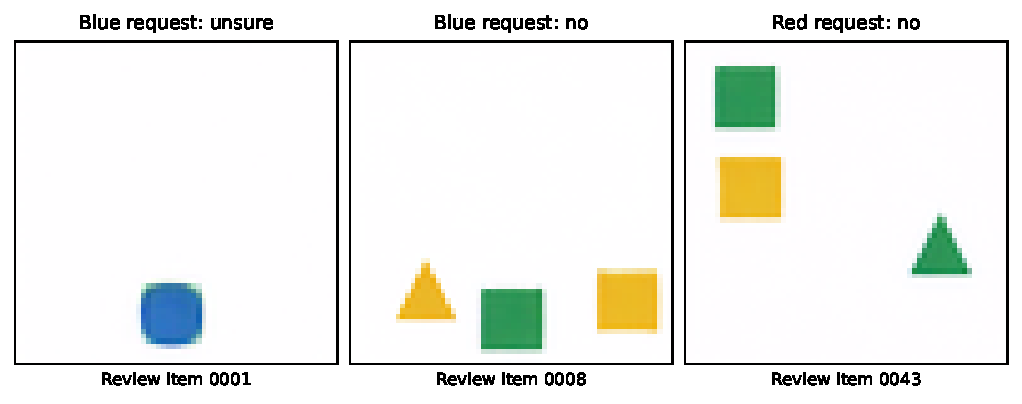
\includegraphics[width=\columnwidth]{figures/review-failures.pdf}\caption{Selected human-reviewed difficult outputs: one unresolved and two negative target-circle labels. Selection is illustrative, not representative.}\label{fig:failures}\end{figure}
\subsection{Additional Instrument-Development Results}
Beyond the matched model pilot, we built a 500-image metadata-labeled synthetic checker set with balanced positive and negative examples, including competing attributes and wrong bindings. On its 100-image test split, the standard checker made 49 decisions and abstained on 51; the experimental checker made 63 decisions and abstained on 37. All accepted decisions agreed with scene metadata in this small synthetic test, which does not establish performance on generated images or human-ambiguous cases. Separately, a foreground segmentation model achieved pooled pixel IoU of 0.9427 on clean and 0.9347 on blur-1 synthetic held-out scenes ($n=100$); this is a pixel metric, not rule-checker accuracy. A new paired-scene generator preserves target and distractor geometry across two- and three-object variants and permits color--shape holdouts. These instruments make further controlled studies possible but do not by themselves validate the exposure hypothesis.

In the network prototype, a localhost CPU-only run of 300,000 scenes per batch setting measured 1,082, 1,061 and 1,060 scenes/s at batch sizes 2, 8 and 16. Separate cross-laptop SSH-tunnel runs of 300 scenes per setting measured 582, 801 and 926 scenes/s on one laptop, and 556, 827 and 514 scenes/s on the other. These include rendering and encoding, use one sub-second trial per setting, and do not measure GPU idle time, physical link capacity or distributed inference speedup. A 4.38 MB checkpoint transfer to the second laptop resumed at 50,000 compressed bytes after a deliberate disconnect and matched the source SHA-256. With that checkpoint, a two-image inference test assigned one job to each GPU; both PNG hashes matched an earlier single-worker run. This small test is not a speed or reproducibility guarantee. A tiny same-host CPU test established local-versus-streamed training parity and streamed checkpoint resume, not inter-machine GPU training equivalence.

\section{Failure Cases and Limitations}
Near-tautological unconstrained spatial predicates make raw relation exposure a weak test of relational competence. Deterministic associations between relation kind and binding patterns confound some template contrasts. The checker has low coverage and lacks negative accepted examples in the first block; a selective always-positive checker would also agree on this particular accepted subset. Identical returned review files alone cannot verify reviewer identities, and the team confirmed independent reviews for the second block. The exposure designs remain sensitive to the chosen rule distribution, estimated marginals and model specification. The four-cell study concerns object complexity and imbalance, not a direct intervention on joint versus marginal exposure. The initial 1,000-update run was continued with restored model, EMA and optimizer but a fresh RNG state; subsequent checkpoints include RNG state. Two training-seed blocks share one dataset realization per cell in a small synthetic domain; none of these results validates natural-image generalization to other domains.
\section{Conclusion and Future Work}
We built and measured the components for a controlled investigation of compositional exposure and obtained preliminary feasibility evidence from two training-seed blocks. The main hypothesis remains untested and Stage 0 has not passed. Next steps are to validate the checker with negative examples and coverage targets, improve relation templates, agree on the target rule population, and freeze a design with adequate marginal control and identifiable contrasts before training the exposure-intervention study. Future experiments should counterbalance object color, shape, and role, withhold combinations, vary independent dataset and training seeds, and include negative and adversarial checker cases. A more realistic external dataset and architecture ablations are future work, not current results.
\ifdefined\anonymouspaper
\paragraph{Reproducibility.} An anonymized code and artifact package is needed before any conference submission; this draft does not yet include one.
\else
\paragraph{Reproducibility.} Code and documentation: \url{https://github.com/Space-Dev0/muadib}. Generated outputs and model weights may be excluded from the repository. Experimental protocol and counts are in \texttt{docs/06-mosaic/mosaic-matched-eval-82000.md}; the plots are generated by \texttt{paper/generate\_figures.py}.
\fi
\section*{Impact Statement}
This research studies how training data and evaluation affect the reliability of generative models. Its synthetic findings should not be interpreted as evidence of safety or reliability in consequential domains. Wider use of generated images may amplify existing representational errors; independent audits and domain-specific evaluation remain necessary.
\section*{AI Disclosure Statement}
Generative AI assistants contributed to drafting, code and figure preparation, literature discovery, and internal review. The authors remain responsible for checking all claims, citations, artifacts, and the final manuscript.
\bibliography{references}
\bibliographystyle{icml2027}
\end{document}
